\tikzset{highlight/.style={orange!75!white,line width=6pt,line cap=round}}
%\tikzset{highlight2/.style={tngreen!80,line width=11pt,line cap=round}}
\tikzset{highlight2/.style={tngreen!70!yellow!60,line width=11pt,line cap=round}}
\tikzset{psline/.style={decorate,decoration={amplitude=0.3mm,segment length=2mm,post length=1.5mm,pre length=1.5mm,coil,aspect=0}}}
\tikzset{plainlin/.style={line width=1pt}}
\def\shortendistance{5pt}
\tikzset{plainlin shorten/.style={line width=1pt,shorten >=\shortendistance,shorten <=\shortendistance}}

\tikzset{lin shorten/.style={shorten >=\shortendistance,shorten <=\shortendistance,line width=1pt,decoration={markings, mark=at position 0.5*\pgfdecoratedpathlength+1.8pt with {\arrow{angle 90}}}, postaction={decorate}}}
% Name of file with picture %%%%%%%%%%%%%%%%%%%%%%%%%%%%%%%%%%%%%%%%%%%


\newcommand{\vertexat}[1]{\fill [very thick,draw=white,fill=black] #1 circle (3pt);}

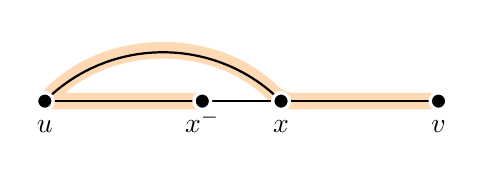
\begin{tikzpicture}

    \coordinate  (u)   at  (0,  1.5);
    \coordinate  (x-)  at  (2,  1.5);
    \coordinate  (x)   at  (3,  1.5);
    \coordinate  (v)   at  (5,  1.5);


    \begin{scope}[opacity=.4]
      \draw [highlight,rounded corners] (x-) to (u) to [out= 45, in=135] (x)
      to  (v);
    \end{scope}


    \draw [thick] (u) to (x-) to (x) to (v);
    \draw [thick] (u) to [out=45,in=135] (x);


    \foreach \nn in {u,x-,x,v} {
      \vertexat{(\nn)};
    }


    \node [anchor=north] at (u) {$u\vphantom{x^-}$};
    \node [anchor=north] at (x-) {$x^-$};
    \node [anchor=north] at (x) {$x\vphantom{x^-}$};
    \node [anchor=north] at (v) {$v\vphantom{x^-}$};
\end{tikzpicture}